% Provenance (never printed): see sources/outline_sources.md (Year 1: internal
% structure of the Earth from seismology; reference model; density, gravity and
% pressure inside the Earth; mantle mineralogy; lithosphere and asthenosphere).
% Curves from figdata/bachelor-1/prem_profiles.py (shared dataset data:prem) and
% figdata/bachelor-1/refraction.py (generic two-layer crust); exercise and problem
% values in the Book 3 scratch calculator calc/ch09.py.
\chapter{De gelaagde aarde}\label{ch:b1:layered-earth}

Op 8 oktober 1909 schudde een aardbeving de Kupa-vallei, ten zuidoosten van Zagreb.
% ledger: skoko:mohorovicic
Andrija Mohorovičić, die het
observatorium daar leidde, verzamelde de seismogrammen die in heel Europa waren geregistreerd en merkte iets vreemds op:
tot enkele honderden kilometers van het epicentrum kwam de eerste trilling op één manier aan, verder weg nam een tweede
soort eerste aankomst het over, alsof een deel van de energie op diepte een snellere weg had gevonden. Hij verklaarde dat
met een grens ongeveer vijftig kilometer diep, waaronder de golven sneller reizen: de basis van de \omterm{def:b1:layered-earth:layers}{korst}. Een eeuw van
dergelijke registraties, miljoenen ervan, heeft die eerste grens veranderd in een \omterm{def:b1:layered-earth:reference-model}{referentiemodel} van de hele aarde,
laag voor laag, met zijn snelheden, zijn dichtheid, zijn zwaartekracht en zijn druk tot aan het middelpunt. Dit hoofdstuk
laat zien hoe een grens uit looptijden wordt gevonden, wat het \omterm{def:b1:layered-earth:reference-model}{referentiemodel} zegt, hoe een dichtheidsprofiel uit
seismische snelheden alleen wordt getekend en gecontroleerd aan de massa en het traagheidsmoment van de aarde, welke
mineralen de \omterm{def:b1:layered-earth:layers}{mantel} op elke diepte vormen, waaruit de kern bestaat, en waar de stijve buitenste schil van de planeet
eindigt.

\begin{recall}
Een P-golf is een compressiegolf, een S-golf een schuifgolf; S-golven gaan niet door vloeistoffen, en de P- en S-schaduwzones
van de kern geven de straal van de vloeibare \omterm{def:b1:layered-earth:layers}{buitenkern} (Boek 2, klas 11). Golven worden op een grens gebroken volgens de wet van
Snellius, $\sin i_1/v_1 = \sin i_2/v_2$ (natuurkunde). In een vloeistof in rust neemt de druk met de diepte toe als
$\mathrm dP = \rho g\,\mathrm dz$ (natuurkunde, eerste jaar universiteit). De \omterm{def:b1:layered-earth:layers}{korst}, de \omterm{def:b1:layered-earth:layers}{mantel} en de kern zijn ingevoerd in
Boek 1 (klas 6).
\end{recall}

\section{Seismische golven in een gelaagde aarde}

De snelheden van seismische golven hangen af van de elastische moduli van het gesteente en van zijn dichtheid. De
natuurkundeboeken leiden ze af uit de vergelijkingen van de continuümelasticiteit; hier worden ze als bekend genomen.

\begin{proposition}[Seismische snelheden]\label{prop:b1:layered-earth:speeds}
In een isotrope elastische vaste stof met dichtheid $\rho$, compressiemodulus $K$ en schuifmodulus
$\mu$ reizen P- en S-golven met
\[
  v_P = \sqrt{\frac{K + \tfrac43\mu}{\rho}}, \qquad v_S = \sqrt{\frac{\mu}{\rho}}.
\]
In een vloeistof is $\mu = 0$: $v_S = 0$ en plant zich geen S-golf voort.
\end{proposition}
\admitted

Aangezien $K$ en $\mu$ positief zijn, geldt altijd $v_P > v_S$: in de \omterm{def:b1:layered-earth:layers}{korst} en \omterm{def:b1:layered-earth:layers}{mantel} van PREM is $v_P$ ongeveer $1.8$ tot $1.9$
keer $v_S$, en P-golven komen eerst aan. Beide snelheden nemen over het algemeen met de diepte toe, omdat druk het gesteente
meer verstijft dan het samendrukt, zodat stralen terugbuigen naar het oppervlak; en op enkele diepten springen zij.

\begin{definition}[Seismische discontinuïteit, Moho, kern-mantelgrens en binnenkerngrens]
\label{def:b1:layered-earth:discontinuity}
Een \emph{seismische discontinuïteit}\index{seismische discontinuïteit} is een oppervlak binnen de aarde waarover de seismische
snelheden, de dichtheid of beide plotseling veranderen, over een dikte die klein is vergeleken met een seismische golflengte. De
\emph{Mohorovičić-discontinuïteit}\index{Mohorovičić-discontinuïteit} (of \emph{Moho}\index{Moho}) is de basis van de \omterm{def:b1:layered-earth:layers}{korst}, waar $v_P$
springt naar ongeveer \qty{8}{km.s^{-1}}. De \emph{kern-mantelgrens}\index{kern-mantelgrens} is het oppervlak tussen de vaste silicaatmantel
en de vloeibare \omterm{def:b1:layered-earth:layers}{buitenkern}; de \emph{binnenkerngrens}\index{binnenkerngrens} is het oppervlak tussen de vloeibare \omterm{def:b1:layered-earth:layers}{buitenkern} en de vaste
\omterm{def:b1:layered-earth:layers}{binnenkern}.
\end{definition}

\subsection{Breking op een laaggrens}

Neem een laag met dikte $h$ en snelheid $v_1$, de \omterm{def:b1:layered-earth:layers}{korst}, op een halfruimte met snelheid $v_2 > v_1$, de \omterm{def:b1:layered-earth:layers}{mantel}, en een bron aan het
oppervlak. Drie golven bereiken een ontvanger op afstand $x$. De directe golf reist in de laag, met $v_1$. De gereflecteerde golf
kaatst op de grens. En een straal die de grens onder de grenshoek $i_c$ raakt, met $\sin i_c = v_1/v_2$, wordt langs haar gebroken, reist
in het snellere medium net eronder met de snelheid $v_2$ en stuurt energie terug omhoog in de laag, onder dezelfde hoek $i_c$ over haar
hele weg.

\begin{definition}[Kopgolf, kruisafstand]\label{def:b1:layered-earth:head-wave}
Een \emph{kopgolf}\index{kopgolf} is de golf die langs een grens reist met de snelheid van het snellere medium eronder en die er
omhoog verlaat onder de grenshoek. De \emph{kruisafstand}\index{kruisafstand} is de afstand van de bron waarbuiten de kopgolf eerder aankomt
dan de directe golf.
\end{definition}

\begin{theorem}[Looptijden over een tweelagige aarde]\label{thm:b1:layered-earth:two-layer}
Over een laag met dikte $h$ en snelheid $v_1$ die rust op een halfruimte met snelheid $v_2 > v_1$, geven een bron aan het oppervlak en een
ontvanger aan het oppervlak op afstand $x$
\[
  t_{\text{direct}} = \frac{x}{v_1}, \qquad
  t_{\text{kop}} = \frac{x}{v_2} + \frac{2h\cos i_c}{v_1}
  \quad (x \ge 2h\tan i_c), \qquad \sin i_c = \frac{v_1}{v_2},
\]
en de \omterm{def:b1:layered-earth:head-wave}{kopgolf} komt het eerst aan voorbij de \omterm{def:b1:layered-earth:head-wave}{kruisafstand}
\[
  x_c = 2h\sqrt{\frac{v_2 + v_1}{v_2 - v_1}}.
\]
\end{theorem}

\begin{proof}
De \omterm{def:b1:layered-earth:head-wave}{kopgolf} gaat onder de hoek $i_c$ door de laag omlaag, een pad van lengte $h/\cos i_c$, loopt langs de grens over de afstand
$x - 2h\tan i_c$, en komt langs een pad van lengte $h/\cos i_c$ omhoog. Haar looptijd is
\[
  t_{\text{kop}} = \frac{2h}{v_1\cos i_c} + \frac{x - 2h\tan i_c}{v_2}
  = \frac{x}{v_2} + \frac{2h}{v_1\cos i_c}\Bigl(1 - \frac{v_1\sin i_c}{v_2}\Bigr)
  = \frac{x}{v_2} + \frac{2h}{v_1\cos i_c}\,(1 - \sin^2 i_c),
\]
dat is $x/v_2 + 2h\cos i_c/v_1$. Het pad bestaat alleen als de horizontale afstand positief is, $x \ge 2h\tan i_c$. De twee tijden zijn
gelijk wanneer $x(1/v_1 - 1/v_2) = 2h\cos i_c/v_1$; met $\cos i_c = \sqrt{v_2^2 - v_1^2}/v_2$,
\[
  x\,\frac{v_2 - v_1}{v_1 v_2} = \frac{2h\sqrt{(v_2 - v_1)(v_2 + v_1)}}{v_1 v_2},
\]
wat $x_c$ geeft. Voorbij dat punt ligt de lijn van de \omterm{def:b1:layered-earth:head-wave}{kopgolf}, met de kleinere helling $1/v_2$, onder de lijn van de directe golf.
\end{proof}

Op een grafiek van looptijd tegen afstand zijn de directe en de \omterm{def:b1:layered-earth:head-wave}{kopgolf} twee rechte lijnen. Hun hellingen zijn de inverse snelheden
$1/v_1$ en $1/v_2$; de lijn van de \omterm{def:b1:layered-earth:head-wave}{kopgolf}, teruggetrokken naar $x = 0$, snijdt de tijdas in de \emph{intercepttijd}
$t_i = 2h\cos i_c/v_1$. De gereflecteerde golf, $t = \sqrt{x^2 + 4h^2}/v_1$, is een hyperbool die de lijn van de \omterm{def:b1:layered-earth:head-wave}{kopgolf} raakt in de
kritieke afstand $2h\tan i_c$, waar de \omterm{def:b1:layered-earth:head-wave}{kopgolf} ontstaat (\cref{exo:b1:layered-earth:10}).

\begin{omfigure}
\begin{tabular}{@{}c@{}}
\begin{tikzpicture}
\begin{axis}[width=0.86\linewidth, axis equal image, xmin=0, xmax=260, ymin=-62, ymax=8,
  axis x line=top, axis y line=left, axis line style={-}, clip=false,
  ylabel={diepte (km)}, ytick={-60,-35,0},
  yticklabels={60,35,0}, tick label style={font=\scriptsize}, label style={font=\small}]
\fill[brown!12] (axis cs:0,0) rectangle (axis cs:260,-35);
\fill[orange!18] (axis cs:0,-35) rectangle (axis cs:260,-62);
\draw[black!60] (axis cs:0,-35) -- (axis cs:260,-35);
\addplot[very thick, blue!70!black] table[x=x, y=z, unbounded coords=jump,
  restrict expr to domain={\coordindex}{0:1}] {figdata/out/bachelor-1-refraction-rays.dat};
\addplot[thick, dashed, green!45!black] table[x=x, y=z, unbounded coords=jump,
  restrict expr to domain={\coordindex}{3:5}] {figdata/out/bachelor-1-refraction-rays.dat};
\addplot[very thick, red!75!black] table[x=x, y=z, unbounded coords=jump,
  restrict expr to domain={\coordindex}{7:10}] {figdata/out/bachelor-1-refraction-rays.dat};
\node[font=\scriptsize, anchor=north west] at (axis cs:2,-36) {mantel, $v_2 = \qty{8.0}{km.s^{-1}}$};
\node[font=\scriptsize, anchor=center] at (axis cs:125,-17) {korst, $v_1 = \qty{6.0}{km.s^{-1}}$, $h = \qty{35}{km}$};
\node[font=\scriptsize, red!75!black, anchor=north] at (axis cs:150,-36) {kopgolf langs de Moho};
\node[font=\scriptsize, green!45!black, anchor=south] at (axis cs:40,-20) {gereflecteerd};
\node[font=\scriptsize, blue!70!black, anchor=north] at (axis cs:125,-1) {direct};
\fill (axis cs:0,0) circle (2pt);
\end{axis}
\end{tikzpicture}\\[2pt]
{\small (a) stralenpaden (afstand in km)}\\[6pt]
\begin{tikzpicture}
\begin{axis}[omrecord, width=0.86\linewidth, height=6.0cm, xmin=0, xmax=400, ymin=0, ymax=70,
  xlabel={afstand $x$ (km)}, ylabel={looptijd $t$ (s)}, tick label style={font=\scriptsize},
  label style={font=\small}, clip=false,
  legend style={font=\scriptsize, at={(0.03,0.97)}, anchor=north west, draw=none, fill=white, fill opacity=0.85}]
\addplot[very thick, blue!70!black] table[x=x, y=t_direct] {figdata/out/bachelor-1-refraction-times.dat};
\addlegendentry{direct, helling $1/v_1$}
\addplot[thick, dashed, green!45!black] table[x=x, y=t_reflected] {figdata/out/bachelor-1-refraction-times.dat};
\addlegendentry{gereflecteerd}
\addplot[very thick, red!75!black, unbounded coords=jump] table[x=x, y=t_head] {figdata/out/bachelor-1-refraction-times.dat};
\addlegendentry{kopgolf, helling $1/v_2$}
\addplot[thin, dotted, red!75!black, domain=0:79.37] {x/8 + 7.717};
\draw[black!60, densely dashed] (axis cs:185.2,0) -- (axis cs:185.2,30.87);
\node[font=\scriptsize, anchor=north west] at (axis cs:187,8) {$x_c = \qty{185}{km}$};
\node[font=\scriptsize, anchor=east, red!75!black] at (axis cs:-3,7.7) {$t_i$};
\end{axis}
\end{tikzpicture}\\[2pt]
{\small (b) looptijden}
\end{tabular}

\par\smallskip{\small Breking over een \omterm{def:b1:layered-earth:layers}{korst} van \qty{35}{km} dik, bij \qty{6.0}{km.s^{-1}}, op een \omterm{def:b1:layered-earth:layers}{mantel} bij \qty{8.0}{km.s^{-1}}
((a) op ware schaal). (a) De directe golf loopt langs het oppervlak; de gereflecteerde golf die getekend is, is de golf die de \omterm{def:b1:layered-earth:discontinuity}{Moho}
onder de grenshoek raakt, \ang{48.6}; de \omterm{def:b1:layered-earth:head-wave}{kopgolf} loopt langs de \omterm{def:b1:layered-earth:discontinuity}{Moho} en keert onder die hoek terug. (b) Aankomsttijden: de \omterm{def:b1:layered-earth:head-wave}{kopgolf} verschijnt
op de kritieke afstand, \qty{79}{km}, rakend aan de reflectie, en haalt de directe golf in op de \omterm{def:b1:layered-earth:head-wave}{kruisafstand}, \qty{185}{km}. De gestippelde
verlenging geeft de intercepttijd $t_i = \qty{7.7}{s}$.}
\end{omfigure}

\begin{method}[De diepte van een grens uit een breking-profiel]\label{met:b1:layered-earth:moho}
\begin{enumerate}
  \item Zet de eerste aankomsttijden uit tegen de afstand, en pas één rechte lijn door de aankomsten dicht bij de bron en een andere door de verre.
  \item De inverse hellingen geven $v_1$ en $v_2$; daarna $\sin i_c = v_1/v_2$.
  \item Lees de intercepttijd $t_i$ van de verre lijn af bij $x = 0$, en reken $h = t_i v_1/(2\cos i_c)$ uit; controleer met de \omterm{def:b1:layered-earth:head-wave}{kruisafstand},
        $h = \tfrac12 x_c\sqrt{(v_2 - v_1)/(v_2 + v_1)}$.
  \item Een grens wordt alleen gevonden als $v_2 > v_1$: een langzamere laag onder een snellere geeft geen \omterm{def:b1:layered-earth:head-wave}{kopgolf} en blijft verborgen.
\end{enumerate}
\end{method}

Mohorovičić' twee soorten eerste aankomst waren precies deze twee lijnen: de directe golf in de \omterm{def:b1:layered-earth:layers}{korst} dicht bij de bron, de \omterm{def:b1:layered-earth:head-wave}{kopgolf} langs de
bovenkant van de \omterm{def:b1:layered-earth:layers}{mantel} verder weg. Zijn schatting van de dikte van de \omterm{def:b1:layered-earth:layers}{korst} in dat gebied, \qty{54}{km}, is in grootteorde bevestigd, maar de
diepte van de \omterm{def:b1:layered-earth:discontinuity}{Moho} varieert van plaats tot plaats. Onder de oceanen is de \omterm{def:b1:layered-earth:layers}{korst} slechts ongeveer \qty{5}{km} dik; onder de continenten
gemiddeld ongeveer \qty{30}{km}, en veel dikker onder grote bergketens. Voor zijn \omterm{def:b1:layered-earth:reference-model}{referentiemodel} plaatste PREM de \omterm{def:b1:layered-earth:discontinuity}{Moho} op \qty{11}{km} onder
zeeniveau onder de oceanen en op \qty{35}{km} onder de continenten.
% ledger: skoko:mohorovicic, usgs:crust-thickness, prem:moho-average

\begin{history}[Andrija Mohorovičić]
\begin{minipage}[t]{0.76\linewidth}\vspace{0pt}
% ledger: skoko:mohorovicic
Andrija Mohorovičić (1857--1936) kwam van de meteorologie naar de seismologie: eerst leraar, daarna van 1891 tot 1921 directeur van het
meteorologisch observatorium van Zagreb; zijn laatste meteorologische studie publiceerde hij in 1901. Op de seismogrammen van de aardbeving
in de Kupa-vallei van 8 oktober 1909 vond hij twee afzonderlijke paren van P- en S-fasen: dicht bij de bron kwam de ene soort eerste trilling
het eerst aan, verder weg een andere, die op diepte sneller had gereisd. Zijn lezing van deze twee aankomsten als een directe golf en een golf
die onder een grens was gebroken, leverde de grens op die nu zijn naam draagt, en de eerste meting van de dikte van de \omterm{def:b1:layered-earth:layers}{korst}.
\end{minipage}\hfill
\begin{minipage}[t]{0.2\linewidth}\vspace{0pt}
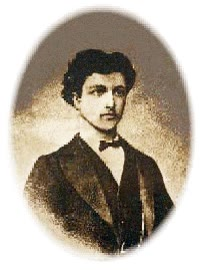
\includegraphics[width=\linewidth]{images/book3/b1-mohorovicic.jpg}

{\scriptsize Andrija Mohorovičić. Publiek domein.}
\end{minipage}
\end{history}

\section{Een referentiemodel van de aarde}

Dezelfde redenering, toegepast op miljoenen looptijden op alle afstanden en op de periodes van de vrije trillingen van de aarde (de hele
planeet klinkt als een klok na een grote aardbeving), geeft de snelheden op elke diepte.

\begin{definition}[Referentiemodel van de aarde]\label{def:b1:layered-earth:reference-model}
Een \emph{referentiemodel van de aarde}\index{referentiemodel van de aarde} is een bolsymmetrische aarde, gegeven als de seismische snelheden $v_P(r)$, $v_S(r)$,
de dichtheid $\rho(r)$ en, in de meest uitgebreide modellen, de dempingsfactor als functies van de straal $r$ alleen, die aansluit op de waargenomen
looptijden, de perioden van de vrije trillingen, de massa van de aarde en haar traagheidsmoment. Het meest gebruikte is PREM, het Preliminary Reference
Earth Model (1981).
\end{definition}

PREM werd aangepast aan de straal \qty{6371}{km}, de massa \qty{5.974e24}{kg} en de \omterm{def:b1:comparative-planetology:moi}{traagheidsmomentfactor} $0.3308$ van de aarde. Het verdeelt de planeet
in enkele gebieden die door discontinuïteiten zijn verbonden, en zijn profielen (figuur hieronder) tonen meteen de belangrijkste lagen.

\begin{definition}[Korst, mantel, buitenkern, binnenkern]\label{def:b1:layered-earth:layers}
De \emph{korst}\index{korst} is de buitenste silicaatlaag boven de \omterm{def:b1:layered-earth:discontinuity}{Moho}. De \emph{mantel}\index{mantel} is de vaste silicaatschil tussen de \omterm{def:b1:layered-earth:discontinuity}{Moho} en de
\omterm{def:b1:layered-earth:discontinuity}{kern-mantelgrens}, op een diepte van ongeveer \qty{2891}{km}. De \emph{buitenkern}\index{buitenkern} is de vloeibare metaalschil tussen de \omterm{def:b1:layered-earth:discontinuity}{kern-mantelgrens}
en de \omterm{def:b1:layered-earth:discontinuity}{binnenkerngrens}, op ongeveer \qty{5150}{km} diepte. De \emph{binnenkern}\index{binnenkern} is de vaste metaalbol eronder, met een straal van ongeveer
\qty{1220}{km}.
\end{definition}

\begin{omfigure}
\begin{tikzpicture}
\begin{axis}[omrecord, omdepth, width=0.62\linewidth, height=5.4cm, xmin=0, xmax=14, ymin=0, ymax=6371,
  xlabel={snelheid (\unit{km.s^{-1}}) of dichtheid (\unit{g.cm^{-3}})}, ylabel={diepte (km)},
  ytick={0,1000,...,6000}, tick label style={font=\scriptsize}, label style={font=\small},
  clip=false, legend style={font=\scriptsize, at={(0.02,0.80)}, anchor=north west, draw=none, fill=white}]
\addplot[very thick, blue!70!black] table[x=vp, y=depth] {figdata/out/bachelor-1-prem_profiles-profiles.dat};
\addlegendentry{$v_P$}
\addplot[very thick, red!75!black] table[x=vs, y=depth] {figdata/out/bachelor-1-prem_profiles-profiles.dat};
\addlegendentry{$v_S$}
\addplot[very thick, black!70, densely dashed] table[x=rho, y=depth] {figdata/out/bachelor-1-prem_profiles-profiles.dat};
\addlegendentry{$\rho$}
\draw[black!35] (axis cs:0,670) -- (axis cs:14,670) node[right, font=\scriptsize, black] {670 km};
\draw[black!35] (axis cs:0,2891) -- (axis cs:14,2891) node[right, font=\scriptsize, black] {kern-mantelgrens};
\draw[black!35] (axis cs:0,5149.5) -- (axis cs:14,5149.5) node[right, font=\scriptsize, black] {binnenkerngrens};
\node[font=\scriptsize, anchor=west] at (axis cs:14,1700) {mantel};
\node[font=\scriptsize, anchor=west] at (axis cs:14,4000) {buitenkern (vloeibaar)};
\node[font=\scriptsize, anchor=west] at (axis cs:14,5800) {binnenkern (vast)};
\end{axis}
\end{tikzpicture}

\par\smallskip{\small PREM: de snelheden van P- en S-golven en de dichtheid tegen de diepte. De S-snelheid valt naar nul in de vloeibare \omterm{def:b1:layered-earth:layers}{buitenkern} en
keert klein terug in de vaste \omterm{def:b1:layered-earth:layers}{binnenkern}; op de \omterm{def:b1:layered-earth:discontinuity}{kern-mantelgrens} verdubbelt de dichtheid bijna terwijl $v_P$ van 13.7 naar \qty{8.1}{km.s^{-1}} daalt;
de sprongen nabij \qty{400}{km} en \qty{670}{km} begrenzen de overgangszone.}
\end{omfigure}

\begin{table}[htbp]
\centering
\footnotesize
\setlength{\tabcolsep}{3pt}
\begin{tabular}{>{\raggedright\arraybackslash}p{0.2\linewidth}rr>{\raggedright\arraybackslash}p{0.47\linewidth}}
\hline
discontinuïteit in PREM & depth (km) & radius (km) & wat verandert \\
\hline
\omterm{def:b1:layered-earth:discontinuity}{Moho} & 24.4 & 6346.6 & \omterm{def:b1:layered-earth:layers}{korst} erboven, peridotiet eronder; $v_P$ 6.8 naar 8.1 \\
discontinuïteit op 220 km & 220 & 6151 & basis van de \omterm{def:b1:layered-earth:lithosphere}{zone met lage snelheid} in PREM \\
discontinuïteit op 400 km & 400 & 5971 & \omterm{def:b1:rock-forming-minerals:groups}{olivijn} naar wadsleyiet (\qty{410}{km} in de meeste studies) \\
discontinuïteit op 670 km & 670 & 5701 & ringwoodiet naar bridgmaniet en ferropericlaas (\qty{660}{km} in de meeste studies) \\
\omterm{def:b1:layered-earth:discontinuity}{kern-mantelgrens} & 2891 & 3480 & silicaat naar vloeibaar ijzer; $v_S$ 7.3 naar 0; $\rho$ 5.57 naar 9.90 \\
\omterm{def:b1:layered-earth:discontinuity}{binnenkerngrens} & 5149.5 & 1221.5 & vloeibaar naar vast ijzer; $v_S$ 0 naar 3.5; $\rho$ 12.17 naar 12.76 \\
\hline
\end{tabular}
\caption{De voornaamste discontinuïteiten van PREM (snelheden in \unit{km.s^{-1}}, dichtheden
in \unit{g.cm^{-3}}). PREM middelt de \omterm{def:b1:layered-earth:layers}{korst} tot \qty{24.4}{km}; echte \omterm{def:b1:layered-earth:layers}{korsten}
variëren van ongeveer \qty{5}{km} onder de oceanen tot vele tientallen kilometers
onder bergketens.}
% ledger: usgs:crust-thickness
\label{tab:b1:layered-earth:prem}
\end{table}

Twee feiten in deze profielen zijn rechtstreeks waargenomen. Het verdwijnen van $v_S$ in de \omterm{def:b1:layered-earth:layers}{buitenkern} is de S-golfschaduw die hierboven is herhaald:
S-golven komen de kern alleen als P-golven binnen, de kern kan geen schuifspanning overbrengen, dus is zij vloeibaar. En de \omterm{def:b1:layered-earth:layers}{binnenkern} laat S-golven door,
langzaam: zij is vast. Dat tweede feit kwam uit zwakke P-aankomsten waar geen P-golf zou moeten zijn.

\begin{history}[Inge Lehmann en de binnenkern]
% ledger: hjortenberg:lehmann
\begin{minipage}[t]{0.76\linewidth}\vspace{0pt}
Inge Lehmann (1888--1993), hoofd van de afdeling seismologie van het Deense geodetisch instituut, bestudeerde de registraties van de aardbeving van Buller
van 1929 in Nieuw-Zeeland en vond P-golven die binnen de schaduwzone aankwamen, waar de kern ze weg had moeten buigen. In een artikel uit 1936 met de kortste
van alle titels, \emph{P$'$}, toonde zij aan dat die verklaard konden worden als de kern een kleinere \omterm{def:b1:layered-earth:layers}{binnenkern} met een hogere P-snelheid bevat, die een deel van
de energie terugstuurt naar het oppervlak. Haar \omterm{def:b1:layered-earth:layers}{binnenkern} is nu bekend als vast, en groeit langzaam wanneer de aarde afkoelt. Zij ontdekte ook de discontinuïteit
nabij \qty{220}{km} die haar naam draagt.
\end{minipage}\hfill
\begin{minipage}[t]{0.2\linewidth}\vspace{0pt}
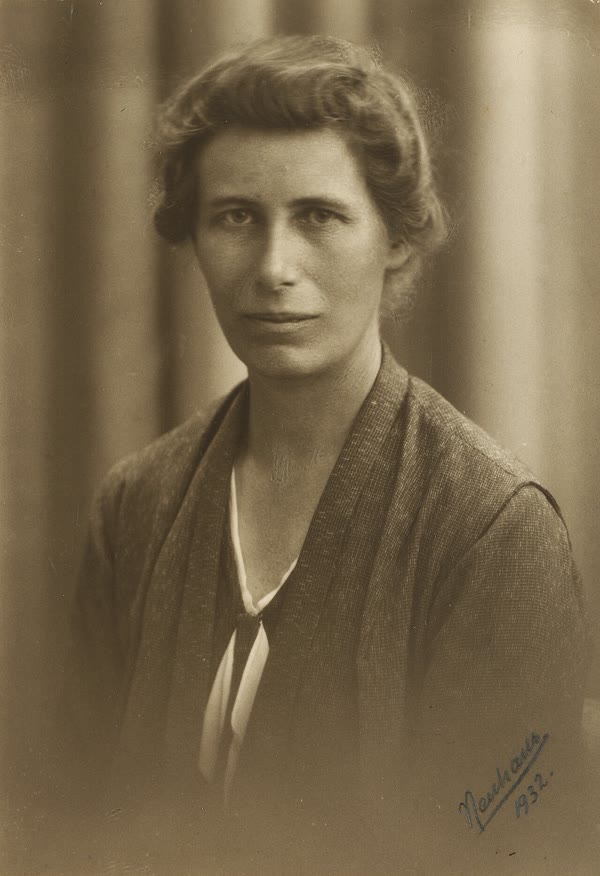
\includegraphics[width=\linewidth]{images/book3/b1-lehmann.jpg}

{\scriptsize Inge Lehmann in 1932, door Even Neuhaus. Publiek domein.}
\end{minipage}
\end{history}

\section{Dichtheid, zwaartekracht en druk uit seismische gegevens}

Seismische snelheden geven twee combinaties van de moduli en de dichtheid, niet de dichtheid zelf. Een derde betrekking komt uit de
aanname dat, binnen een laag van uniforme samenstelling, het gesteente eenvoudig wordt samengedrukt door het gewicht van het
gesteente erboven.

\begin{definition}[Seismische parameter]\label{def:b1:layered-earth:seismic-parameter}
De \emph{seismische parameter}\index{seismische parameter} op een diepte is
\[
  \Phi = v_P^2 - \tfrac43 v_S^2 = \frac{K}{\rho},
\]
de compressiemodulus gedeeld door de dichtheid, berekend uit de twee seismische snelheden alleen (\cref{prop:b1:layered-earth:speeds}).
\end{definition}

\begin{theorem}[Vergelijking van Adams--Williamson]\label{thm:b1:layered-earth:adams-williamson}
In een gebied van uniforme samenstelling, in hydrostatisch evenwicht, adiabatisch samengedrukt, varieert de dichtheid met de straal als
\[
  \frac{\mathrm d\rho}{\mathrm dr} = -\frac{\rho(r)\,g(r)}{\Phi(r)},
\]
waarin $g(r)$ de zwaartekracht op de straal $r$ is.
\end{theorem}

\begin{proof}
Hydrostatisch evenwicht geeft $\mathrm dP/\mathrm dr = -\rho g$ (herschreven met $\mathrm dz = -\mathrm dr$). De compressiemodulus is gedefinieerd door
$K = \rho\,\mathrm dP/\mathrm d\rho$ voor de compressie die aan de orde is; voor een gesteente van vaste samenstelling dat zonder warmte-uitwisseling
wordt samengedrukt, is het de adiabatische modulus die de seismische golven meten, dus $\mathrm d\rho/\mathrm dP = \rho/K$.
Volgens de kettingregel,
\[
  \frac{\mathrm d\rho}{\mathrm dr} = \frac{\mathrm d\rho}{\mathrm dP}\,
  \frac{\mathrm dP}{\mathrm dr} = \frac{\rho}{K}\,(-\rho g) = -\frac{\rho g}{K/\rho}
  = -\frac{\rho g}{\Phi}. \qedhere
\]
\end{proof}

De vergelijking faalt op een discontinuïteit, waar de samenstelling of de kristalstructuur verandert, en overal waar de temperatuur van de adiabaat
afwijkt; maar tussen de discontinuïteiten verklaart zij de waargenomen toename van de dichtheid met de diepte zeer goed (paneel (c) van de figuur
hieronder). Door met een dichtheid aan de bovenkant van elk gebied te beginnen, naar beneden te integreren en de beginwaarden bij te stellen tot de massa en het
traagheidsmoment kloppen, werden zo de eerste dichtheidsmodellen gebouwd. De twee globale getallen zijn integralen van de dichtheid.

\begin{proposition}[Massa, zwaartekracht, druk en traagheidsmoment]
\label{prop:b1:layered-earth:integrals}
Voor een bolsymmetrische aarde met straal $R$ en dichtheid $\rho(r)$ zijn de massa binnen de straal $r$, de zwaartekracht, de druk en het traagheidsmoment
om een as door het middelpunt
\[
  m(r) = \int_0^r 4\pi s^2\rho(s)\,\mathrm ds, \quad
  g(r) = \frac{G\,m(r)}{r^2}, \quad
  P(r) = \int_r^R \rho(s)\,g(s)\,\mathrm ds, \quad
  I = \frac{8\pi}{3}\int_0^R \rho(r)\,r^4\,\mathrm dr.
\]
\end{proposition}

\begin{proof}
Een dunne schil met straal $s$ en dikte $\mathrm ds$ heeft het volume $4\pi s^2\,\mathrm ds$, vandaar de eerste integraal. De zwaartekracht van een bolsymmetrisch
lichaam buiten een straal is die van zijn massa binnen die straal, geconcentreerd in het middelpunt, en de schillen buiten $r$ trekken zonder netto kracht
(de schilstelling, uit de natuurkundeboeken aanvaard); vandaar $g(r)$. De hydrostatische vergelijking vanaf het oppervlak, waar $P = 0$, integrerend geeft
$P(r)$. Voor het traagheidsmoment heeft een dunne bolschil van massa $\mathrm dm$ en straal $r$, om de drie assen $x$, $y$, $z$, momenten waarvan de som
$\int (y^2 + z^2) + (z^2 + x^2) + (x^2 + y^2)\,\mathrm dm = 2r^2\,\mathrm dm$ is; door symmetrie zijn de drie gelijk, dus elk is $\tfrac23 r^2\,\mathrm dm$. Met
$\mathrm dm = 4\pi r^2\rho\,\mathrm dr$ geeft het optellen van de schillen $I$.
\end{proof}

Voor een bol met uniforme dichtheid is $I = \tfrac{8\pi}{15}\rho R^5 = 0.4\,MR^2$. De factor $I/MR^2 = 0.3308$ van de aarde is kleiner: haar massa is naar het
midden geconcentreerd, wat het eerste argument is voor een dichte kern. Berekend uit de dichtheid van PREM alleen, geven de integralen een massa van
\qty{5.976e24}{kg} (\qty{0.06}{\percent} boven de gemeten \qty{5.972e24}{kg}), een factor $0.3309$, en een centrale druk van \qty{364}{GPa}, de waarde die bij PREM
is getabelleerd tot op \qty{0.1}{\percent}.

\begin{omfigure}
\begin{tabular}{@{}c@{\hspace{2mm}}c@{\hspace{2mm}}c@{}}
\begin{tikzpicture}
\begin{axis}[omrecord, omdepth, width=0.35\linewidth, height=7.0cm, xmin=0, xmax=12, ymin=0, ymax=6371,
  xlabel={$g$ (\unit{m.s^{-2}})}, ylabel={diepte (km)}, ytick={0,1000,...,6000}, xtick={0,4,8,12},
  tick label style={font=\scriptsize}, label style={font=\small}]
\addplot[very thick, blue!70!black] table[x=g, y=depth] {figdata/out/bachelor-1-prem_profiles-functionals.dat};
\draw[black!35] (axis cs:0,2891) -- (axis cs:12,2891);
\draw[black!35] (axis cs:0,5149.5) -- (axis cs:12,5149.5);
\node[font=\scriptsize, anchor=south west] at (axis cs:0.3,2891) {CMB};
\node[font=\scriptsize, anchor=south west] at (axis cs:0.3,5149.5) {ICB};
\end{axis}
\end{tikzpicture}
&
\begin{tikzpicture}
\begin{axis}[omrecord, omdepth, width=0.35\linewidth, height=7.0cm, xmin=0, xmax=400, ymin=0, ymax=6371,
  xlabel={$P$ (GPa)}, ytick={0,1000,...,6000}, yticklabels={}, xtick={0,200,400},
  tick label style={font=\scriptsize}, label style={font=\small}]
\addplot[very thick, red!75!black] table[x=P, y=depth] {figdata/out/bachelor-1-prem_profiles-functionals.dat};
\draw[black!35] (axis cs:0,2891) -- (axis cs:400,2891);
\draw[black!35] (axis cs:0,5149.5) -- (axis cs:400,5149.5);
\node[font=\scriptsize, anchor=south west] at (axis cs:150,2891) {\qty{136}{GPa}};
\node[font=\scriptsize, anchor=south east] at (axis cs:290,5149.5) {\qty{329}{GPa}};
\end{axis}
\end{tikzpicture}
&
\begin{tikzpicture}
\begin{axis}[omrecord, omdepth, width=0.35\linewidth, height=7.0cm, xmin=2, xmax=14, ymin=0, ymax=6371,
  xlabel={$\rho$ (\unit{g.cm^{-3}})}, ytick={0,1000,...,6000}, yticklabels={}, xtick={2,6,10,14},
  tick label style={font=\scriptsize}, label style={font=\small},
  legend style={font=\scriptsize, at={(0.97,0.97)}, anchor=north east, draw=none, fill=white}]
\addplot[very thick, black!55] table[x=rho, y=depth] {figdata/out/bachelor-1-prem_profiles-profiles.dat};
\addlegendentry{PREM}
\addplot[only marks, mark=o, mark size=1.4pt, orange!85!black, each nth point=15, unbounded coords=discard]
  table[x=rho_aw, y=depth] {figdata/out/bachelor-1-prem_profiles-adams.dat};
\addlegendentry{Adams--Williamson}
\end{axis}
\end{tikzpicture}
\\[2pt]
{\small (a) zwaartekracht} & {\small (b) druk} & {\small (c) zelfcompressie}
\end{tabular}

\par\smallskip{\small Binnen in de aarde, uit PREM. (a) en (b) Zwaartekracht en druk, berekend uit de dichtheid van PREM met
\cref{prop:b1:layered-earth:integrals}: de zwaartekracht blijft dicht bij \qty{10}{m.s^{-2}} door de \omterm{def:b1:layered-earth:layers}{mantel}, bereikt een piek van
\qty{10.7}{m.s^{-2}} op de \omterm{def:b1:layered-earth:discontinuity}{kern-mantelgrens} (CMB) en daalt tot nul in het middelpunt; de druk bereikt \qty{136}{GPa} op de CMB, \qty{329}{GPa}
op de \omterm{def:b1:layered-earth:discontinuity}{binnenkerngrens} (ICB) en \qty{364}{GPa} in het middelpunt. (c) De vergelijking van Adams--Williamson, naar beneden geïntegreerd vanaf de dichtheid van
PREM bij \qty{771}{km} en aan de bovenkant van de \omterm{def:b1:layered-earth:layers}{buitenkern} met de snelheden en zwaartekracht van PREM (cirkels), volgt PREM binnen \qty{0.2}{\percent}:
daar is de toename van de dichtheid de samendrukking van een uniform materiaal; de sprongen niet.}
\end{omfigure}

Dat de zwaartekracht naar beneden in de \omterm{def:b1:layered-earth:layers}{mantel} toeneemt, is een rechtstreeks gevolg van de dichte kern: de massa die binnen de straal overblijft,
neemt langzamer af dan $r^2$. Door de \omterm{def:b1:layered-earth:layers}{mantel} verandert $g$ nauwelijks, en de druk neemt bijna lineair met de diepte toe, met ongeveer
\qty{4.7}{GPa} per honderd kilometer.


\section{De mantel: één gesteente, meerdere mineraalassemblages}

De bovenste \omterm{def:b1:layered-earth:layers}{mantel} is peridotiet, bekend uit de brokstukken die vulkanen naar boven brengen en uit stukken \omterm{def:b1:layered-earth:layers}{mantel} die op continenten zijn geschoven: ongeveer de
helft tot drie vijfde \omterm{def:b1:rock-forming-minerals:groups}{olivijn} naar volume (\qtyrange{49}{62}{\percent} in de voorgestelde samenstellingen), de rest pyroxenen en een aluminiumrijk \omterm{def:b1:rock-forming-minerals:mineral}{mineraal}
(\omterm{def:b1:rock-forming-minerals:groups}{plagioklaas}, spinel of \omterm{def:b1:rock-forming-minerals:groups}{granaat}, afhankelijk van de diepte). De druk die met de diepte toeneemt, verandert deze samenstelling niet, maar dwingt haar atomen tot
dichtere rangschikkingen: \omterm{def:b1:rock-forming-minerals:polymorph}{polymorfen} (\cref{ch:b1:rock-forming-minerals}) verschijnen de een na de ander.

\begin{definition}[Overgangszone van de mantel]\label{def:b1:layered-earth:transition-zone}
De \emph{overgangszone van de mantel}\index{overgangszone van de mantel} is het deel van de \omterm{def:b1:layered-earth:layers}{mantel} tussen de \omterm{def:b1:layered-earth:discontinuity}{seismische discontinuïteiten} nabij
\qty{410}{km} en \qty{660}{km} diepte, waarin \omterm{def:b1:rock-forming-minerals:groups}{olivijn} van de bovenste \omterm{def:b1:layered-earth:layers}{mantel} wordt vervangen door zijn dichtere \omterm{def:b1:rock-forming-minerals:polymorph}{polymorfen}, wadsleyiet en daarna
ringwoodiet. Erboven ligt de bovenste \omterm{def:b1:layered-earth:layers}{mantel}; eronder de onderste \omterm{def:b1:layered-earth:layers}{mantel}, tot de \omterm{def:b1:layered-earth:discontinuity}{kern-mantelgrens}.
\end{definition}

Op ongeveer \qty{410}{km} (\qty{14}{GPa}) wordt \omterm{def:b1:rock-forming-minerals:groups}{olivijn} \ce{(Mg,Fe)2SiO4} wadsleyiet, met dezelfde formule; nabij \qty{520}{km} (\qty{17.5}{GPa}) wordt wadsleyiet tot
ringwoodiet; de pyroxenen lossen op in een siliciumrijk \omterm{def:b1:rock-forming-minerals:groups}{granaat}, majoriet, totdat het \omterm{def:b1:rock-forming-minerals:groups}{granaat} ze tegen het midden van de overgangszone alle bevat, zodat de zone iets
meer dan de helft olivijnpolymorfen is en de rest \omterm{def:b1:rock-forming-minerals:groups}{granaat}. Op ongeveer \qty{660}{km}, bij een druk nabij \qty{24}{GPa}, valt ringwoodiet uiteen in
twee mineralen, geschreven voor het magnesiumrijke \omterm{def:b1:rock-forming-minerals:solid-solution}{eindlid}
\[
  \ce{Mg2SiO4 -> MgSiO3 + MgO}:
\]
bridgmaniet, \ce{(Mg,Fe)SiO3} met de structuur van perovskiet, en ferroperiklaas, \ce{(Mg,Fe)O}. Een onderste \omterm{def:b1:layered-earth:layers}{mantel} van dezelfde samenstelling als de
bovenste \omterm{def:b1:layered-earth:layers}{mantel} bestaat voor ongeveer \qty{75}{\percent} uit bridgmaniet, \qty{17}{\percent} ferroperiklaas en \qty{8}{\percent} calciumsilicaatperovskiet
naar volume, en past op de dichtheden en snelheden van het \omterm{def:b1:layered-earth:reference-model}{referentiemodel}. Bridgmaniet is daarom het meest voorkomende \omterm{def:b1:rock-forming-minerals:mineral}{mineraal} van de aarde; het kreeg
zijn naam pas in 2014, nadat natuurlijke korrels waren beschreven in een zwaar geschokte meteoriet.
% ledger: frost:mantle-transitions, sun:lower-mantle, tschauner:bridgmanite

Elke verandering levert dichtere mineralen op, en verhoogt daarmee de dichtheid en de seismische snelheden: de overgangen zijn de discontinuïteiten van de
profielen (figuur hieronder). Hun diepten liggen niet vast. Een fasewijziging gebeurt bij een druk die van de temperatuur afhangt, en de helling van die
afhankelijkheid (de Clapeyron-helling, die in Boek 4 aan bod komt) verschuift de \qty{410}{km}-discontinuïteit omhoog en de
\qty{660}{km}-discontinuïteit omlaag in het koude gesteente van een zinkende plaat. Het in kaart brengen van de topografie van de discontinuïteiten is
één manier om koude en warme gebieden in de \omterm{def:b1:layered-earth:layers}{mantel} te vinden.

\begin{omfigure}
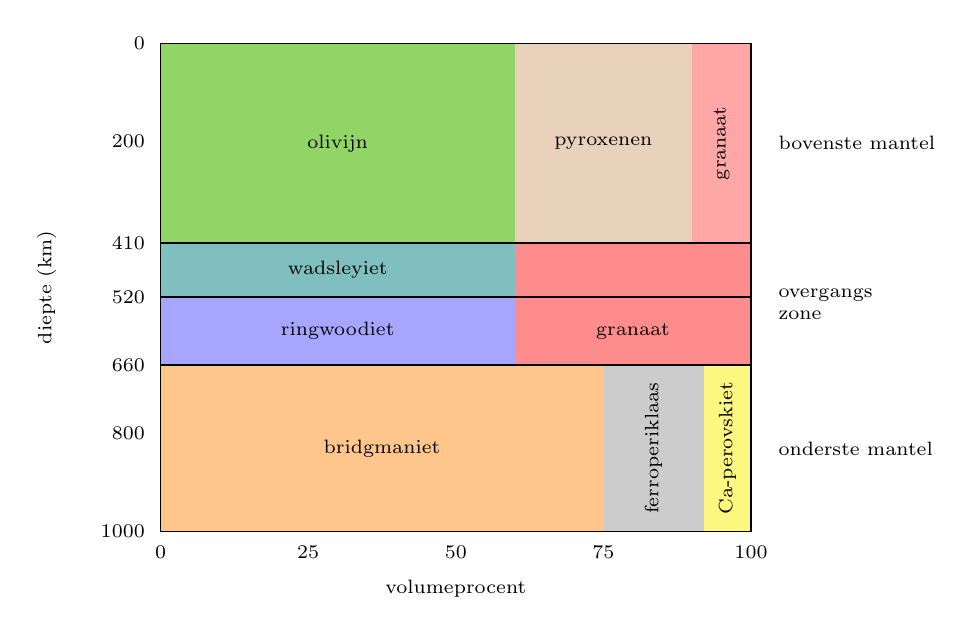
\begin{tikzpicture}[x=0.075mm, y=-0.062mm, font=\scriptsize]
% schematic volume fractions (ledger frost:mantle-transitions, sun:lower-mantle)
\def\W{1000}
% upper mantle 0-410: olivine 60, pyroxenes 30, garnet 10
\fill[green!45!olive!60] (0,0) rectangle (600,410);
\fill[brown!35] (600,0) rectangle (900,410);
\fill[red!35] (900,0) rectangle (1000,410);
% 410-520 wadsleyite 60, garnet 40 ; 520-660 ringwoodite 60, garnet 40
\fill[teal!50] (0,410) rectangle (600,520);
\fill[blue!35] (0,520) rectangle (600,660);
\fill[red!45] (600,410) rectangle (1000,660);
% 660-1000 bridgmanite 75, ferropericlase 17, Ca-perovskite 8
\fill[orange!45] (0,660) rectangle (750,1000);
\fill[gray!40] (750,660) rectangle (920,1000);
\fill[yellow!50] (920,660) rectangle (1000,1000);
\draw (0,0) rectangle (1000,1000);
\foreach \d in {410,520,660} \draw[thick] (0,\d) -- (1000,\d);
\node at (300,205) {olivijn};
\node[align=center] at (750,205) {pyroxenen};
\node[rotate=90] at (950,205) {granaat};
\node at (300,465) {wadsleyiet};
\node at (300,590) {ringwoodiet};
\node[align=center] at (800,590) {granaat};
\node at (375,830) {bridgmaniet};
\node[rotate=90, align=center] at (835,830) {ferroperiklaas};
\node[rotate=90] at (960,830) {Ca-perovskiet};
\foreach \d in {0,200,410,520,660,800,1000} \node[anchor=east] at (-10,\d) {\d};
\node[rotate=90, anchor=south] at (-160,500) {diepte (km)};
\foreach \p in {0,25,50,75,100} \node[anchor=north] at (\p*10,1010) {\p};
\node[anchor=north] at (500,1080) {volumeprocent};
\node[anchor=west, align=left] at (1030,205) {bovenste mantel};
\node[anchor=west, align=left] at (1030,535) {overgangs\\zone};
\node[anchor=west, align=left] at (1030,830) {onderste mantel};
\end{tikzpicture}

\par\smallskip{\small De mineralen van een peridotietmantel met de diepte, als volumefracties (schematisch: de grenzen zijn scherp getekend, en de fracties
zijn ronde waarden binnen de bereiken die in de tekst worden genoemd). De samenstelling verandert niet; de mineralen wel, op ongeveer 410, 520 en
\qty{660}{km}.}
\end{omfigure}

Aan de onderkant van de \omterm{def:b1:layered-earth:layers}{mantel} heeft de laag die D$''$ wordt genoemd (D dubbel accent, een naam die uit een vroeg model van de aarde is overgehouden) een
gradiënt van de snelheid die afwijkt van de rest van de onderste \omterm{def:b1:layered-earth:layers}{mantel}; PREM kent haar de onderste \qty{150}{km} van de \omterm{def:b1:layered-earth:layers}{mantel} toe. Zij is seismisch heterogeen:
plekken van zeer lage snelheid, steile gradiënten, reflectoren. Zij wordt beschouwd als een grenslaag tussen de hete kern en de \omterm{def:b1:layered-earth:layers}{mantel}, en misschien als een
begraafplaats van oude platen.
% ledger: prem:dpp

\section{De kern}

De kern bestaat voornamelijk uit ijzer. Haar dichtheid, haar snelheden en haar vermogen om een magnetisch veld op te wekken wijzen allemaal op een metaal, en
ijzer is van de dichte elementen die meteorieten en de zon laten zien verreweg het overvloedigst. Nikkel, rijk in ijzermeteorieten,
gaat ermee samen. Maar de kern is niet zuiver ijzer--nikkel.
\begin{itemize}
  \item De kern is \qtyrange{5}{10}{\percent} minder dicht dan zuiver ijzer bij dezelfde druk en temperatuur zou zijn: zij moet lichte elementen bevatten,
        waarvan silicium, zwavel, koolstof, zuurstof en waterstof de kandidaten zijn.
  \item De dichtheid springt met ongeveer \qty{4.5}{\percent} op de \omterm{def:b1:layered-earth:discontinuity}{binnenkerngrens}, te veel voor het stollen van één en hetzelfde metaal: de \omterm{def:b1:layered-earth:layers}{binnenkern}
        bevat ook lichte elementen, maar minder, enkele procenten tegen \qtyrange{5}{10}{\percent} in de vloeistof.
\end{itemize}
% ledger: badro:core
Het verschil heeft een gevolg. Terwijl de aarde afkoelt --- haar \omterm{def:b1:layered-earth:layers}{mantel} met ongeveer \qty{100}{\degreeCelsius} per miljard jaar op dit moment ---
stolt de vloeistof van de kern op de \omterm{def:b1:layered-earth:layers}{binnenkern}, die groeit, en
% ledger: bellini:cooling
bij het stollen blijft het grootste deel van de lichte elementen in de vloeistof. De lichte vloeistof die aan de onderkant van de \omterm{def:b1:layered-earth:layers}{buitenkern} vrijkomt, stijgt op,
en men denkt dat deze opdrijving helpt de \omterm{def:b1:layered-earth:layers}{buitenkern} te roeren en de dynamo aan te drijven die het magnetische veld van de aarde maakt.

\section{Mechanische lagen: lithosfeer en asthenosfeer}

De lagen hierboven zijn gedefinieerd door samenstelling en fase: \omterm{def:b1:layered-earth:layers}{korst} en \omterm{def:b1:layered-earth:layers}{mantel} zijn verschillende gesteenten, \omterm{def:b1:layered-earth:layers}{buitenkern} en \omterm{def:b1:layered-earth:layers}{binnenkern} verschillende toestanden.
Plaattektoniek heeft een andere indeling nodig, naar sterkte, die de eerste dwarsdoorsnijdt.

\begin{definition}[Lithosfeer, asthenosfeer, zone met lage snelheid]
\label{def:b1:layered-earth:lithosphere}
De \emph{lithosfeer}\index{lithosfeer} is de stijve buitenste schil van de aarde, de \omterm{def:b1:layered-earth:layers}{korst} en de bovenste \omterm{def:b1:layered-earth:layers}{mantel}, die zich over geologische tijden als een sterke laag
gedraagt en in platen verdeeld is. De \emph{asthenosfeer}\index{asthenosfeer} is de zwakkere laag van de bovenste \omterm{def:b1:layered-earth:layers}{mantel} eronder, die vervormt door langzame stroming
en de platen laat bewegen. De \emph{zone met lage snelheid}\index{zone met lage snelheid} is het dieptebereik onder de lithosfeer waar de seismische snelheden, vooral de
S-snelheden, lager zijn dan net erboven en eronder.
\end{definition}

De \omterm{def:b1:layered-earth:lithosphere}{lithosfeer} is geen gesteente maar een temperatuurbereik: mantelperidotiet is sterk waar het koud is en kruipt waar het heet is, en haar basis is ruwweg een
isotherm. Zij is dun onder ruggen, waar hete \omterm{def:b1:layered-earth:layers}{mantel} opstijgt, ongeveer \qty{140}{km} dik onder de oudste oceaanbodem, en \qtyrange{40}{280}{km} dik onder
continenten, het dikst onder oude kratons; de bovenkant van de \omterm{def:b1:layered-earth:lithosphere}{asthenosfeer} ligt op ongeveer \qtyrange{80}{200}{km}. Seismisch toont de \omterm{def:b1:layered-earth:lithosphere}{asthenosfeer} zich als de \omterm{def:b1:layered-earth:lithosphere}{zone
met lage snelheid}, dicht bij haar smeltcondities: in PREM neemt de S-snelheid licht af van de \omterm{def:b1:layered-earth:discontinuity}{Moho} tot \qty{220}{km}, waar zij weer springt. Hoe sterkte van de temperatuur
afhangt, en waarom, is het onderwerp van \cref{ch:b1:stress-strain-rheology}.

\begin{inthefield}[Een seismisch station]
\begin{minipage}[t]{0.55\linewidth}\vspace{0pt}
De looptijden waarop referentiemodellen rusten, komen van permanente stations. Een breedbandseismometer, die grondbewegingen registreert van honderdsten van een seconde
tot uren in periode, staat op een betonnen pijler die op kaal gesteente is gezet en geïsoleerd is van de vloer van de kelder, onder een afdekking die de temperatuur
stabiel houdt: een verandering van een fractie van een graad, een tocht of een voorbijrijdende vrachtwagen zou op de registratie zichtbaar zijn. De datalogger voorziet
elk monster van een tijdstip uit satellieten, en de registraties stromen naar datacentra die ze open delen. Netwerken van zulke stations lokaliseren en dateren elke grote
aardbeving; aankomsttijden die op hun registraties zijn afgelezen, werden omgekeerd tot de snelheden op elke diepte.
\end{minipage}\hfill
\begin{minipage}[t]{0.42\linewidth}\vspace{0pt}
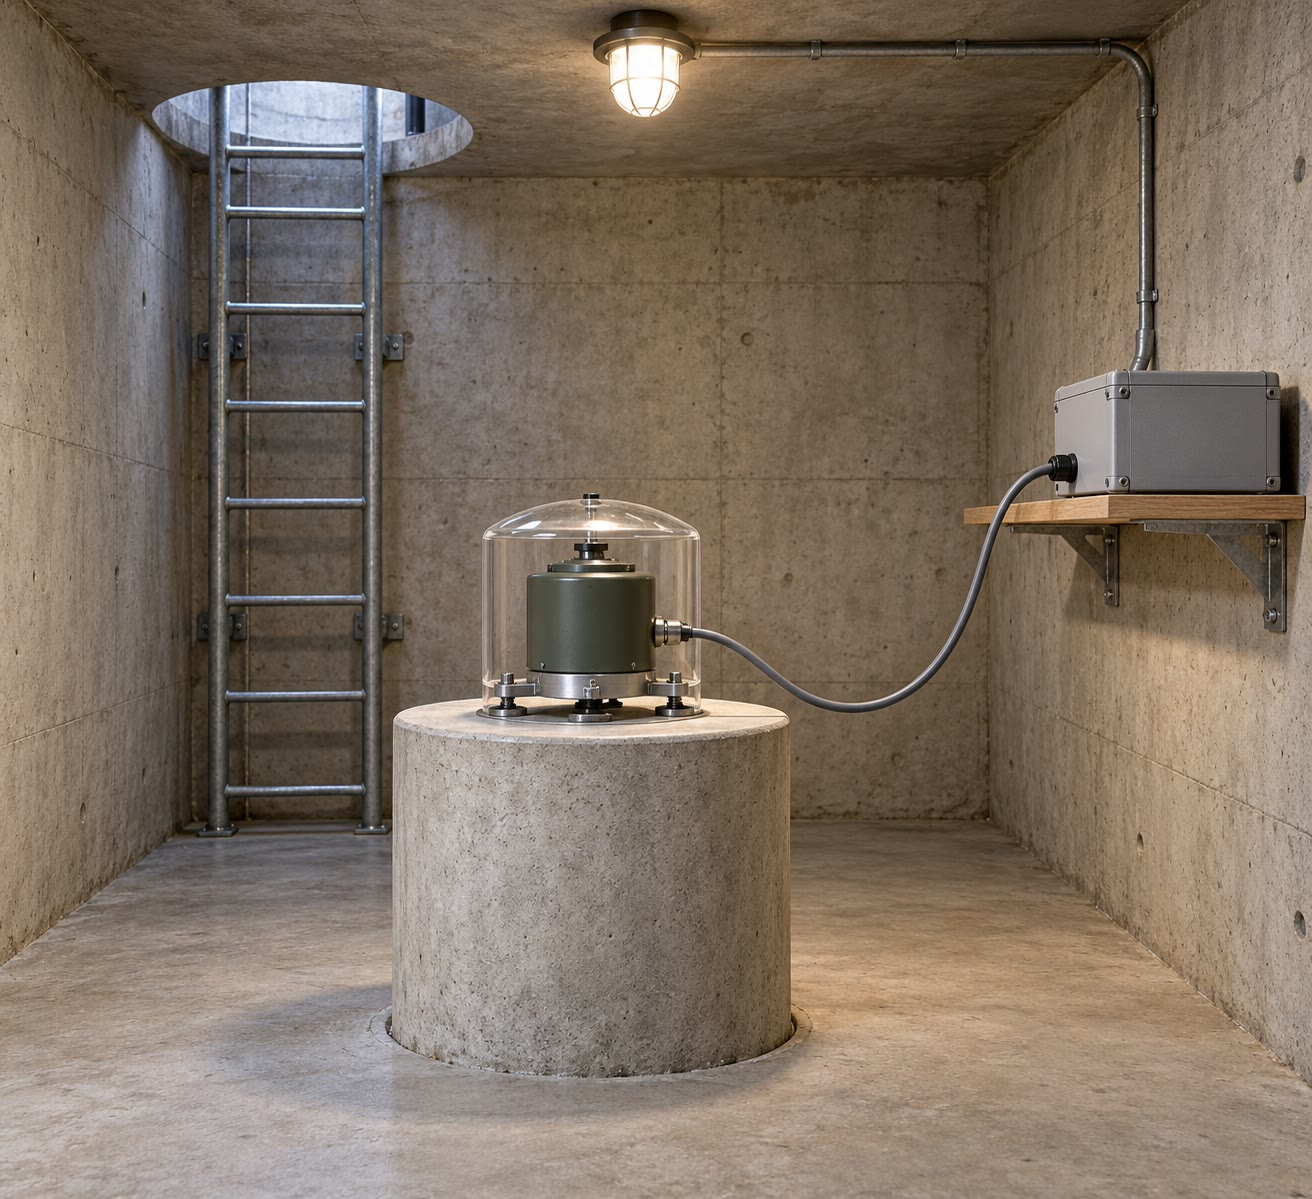
\includegraphics[width=\linewidth]{images/book3/ai/b1-seismometer-vault.jpg}

{\scriptsize Een breedbandseismometer op zijn pijler in een ondergrondse kelder, met de datalogger aan de muur (AI-gegenereerde illustratie).}
\end{minipage}
\end{inthefield}

\section{Oefeningen}

\begin{exercise}[$\star$]\label{exo:b1:layered-earth:1}
Met de straal van PREM $R = \qty{6371}{km}$, $r_{\text{CMB}} = \qty{3480}{km}$ en
$r_{\text{ICB}} = \qty{1221.5}{km}$, bereken de fracties van het volume van de aarde die de kern en de \omterm{def:b1:layered-earth:layers}{binnenkern} innemen.
% ledger: prem:cmb, prem:icb
\end{exercise}

\begin{exercise}[$\star$]\label{exo:b1:layered-earth:2}
Net boven de \omterm{def:b1:layered-earth:discontinuity}{kern-mantelgrens} geeft PREM $v_P = \qty{13.7166}{km.s^{-1}}$,
$v_S = \qty{7.26466}{km.s^{-1}}$, $\rho = \qty{5.56645}{g.cm^{-3}}$; net eronder,
$v_P = \qty{8.06482}{km.s^{-1}}$, $v_S = 0$, $\rho = \qty{9.90349}{g.cm^{-3}}$.
Bereken de \omterm{def:b1:layered-earth:seismic-parameter}{seismische parameter} en de compressiemodulus aan elke kant (in GPa). Wat verandert het meest over de grens?
% ledger: data:prem, prem:cmb
\end{exercise}

\begin{exercise}[$\star$]\label{exo:b1:layered-earth:3}
Een \omterm{def:b1:layered-earth:layers}{korst} van \qty{30}{km} dik, bij \qty{6.2}{km.s^{-1}}, rust op een \omterm{def:b1:layered-earth:layers}{mantel} bij \qty{8.1}{km.s^{-1}}. Bereken de grenshoek, de kritieke afstand en de \omterm{def:b1:layered-earth:head-wave}{kruisafstand}.
\end{exercise}

\begin{exercise}[$\star$]\label{exo:b1:layered-earth:4}
De massa van de kern is \qty{1.94e24}{kg} en haar straal \qty{3480}{km}. Bereken de zwaartekracht op de \omterm{def:b1:layered-earth:discontinuity}{kern-mantelgrens} en vergelijk die met de
zwaartekracht aan het oppervlak, \qty{9.82}{m.s^{-2}}. Waarom is zij groter?
\end{exercise}

\begin{exercise}[$\star\star$]\label{exo:b1:layered-earth:5}
Op een breking-profiel liggen de eerste aankomsten op \qty{10.0}{s} bij \qty{60}{km}, en op \qty{33.3}{s} bij \qty{200}{km} en \qty{45.8}{s} bij
\qty{300}{km}; de lijn door het eerste punt gaat door de oorsprong. Vind $v_1$, $v_2$, de intercepttijd en de diepte van de grens, en controleer het
resultaat met de \omterm{def:b1:layered-earth:head-wave}{kruisafstand}.
\end{exercise}

\begin{exercise}[$\star\star$]\label{exo:b1:layered-earth:6}
Toon aan dat een uniforme bol $I = 0.4\,MR^2$ heeft. Bereken dan de massa en de factor $I/MR^2$ van een aarde met twee lagen: een kern met straal
\qty{3480}{km} en dichtheid \qty{11.0}{g.cm^{-3}} in een \omterm{def:b1:layered-earth:layers}{mantel} met dichtheid \qty{4.45}{g.cm^{-3}}, met $R = \qty{6371}{km}$. Vergelijk met \num{5.972e24} kg en $0.3308$.
\end{exercise}

\begin{exercise}[$\star\star$]\label{exo:b1:layered-earth:7}
Op \qty{1471}{km} diepte geeft PREM $v_P = \qty{12.16}{km.s^{-1}}$, $v_S = \qty{6.673}{km.s^{-1}}$, $\rho = \qty{4.86}{g.cm^{-3}}$, en de zwaartekracht
is \qty{9.9}{m.s^{-2}}. Bereken de dichtheidsgradiënt die de vergelijking van Adams--Williamson geeft, in \unit{g.cm^{-3}} per \qty{1000}{km}, en vergelijk
die met de dichtheden van PREM, \num{4.844} op \qty{1471}{km} en \num{5.357} op \qty{2471}{km}.
% ledger: data:prem
\end{exercise}

\begin{exercise}[$\star\star$]\label{exo:b1:layered-earth:8}
Schat de druk op \qty{670}{km} diepte uit een gemiddelde dichtheid van \qty{3.57}{g.cm^{-3}} en een zwaartekracht van \qty{9.9}{m.s^{-2}}. Welke mineraalovergang
wordt daar verwacht?
% ledger: frost:mantle-transitions
\end{exercise}

\begin{exercise}[$\star\star$]\label{exo:b1:layered-earth:9}
De gemiddelde dichtheid van de \omterm{def:b1:layered-earth:layers}{buitenkern} in PREM is \qty{10.90}{g.cm^{-3}}; op de \omterm{def:b1:layered-earth:discontinuity}{binnenkerngrens} is haar dichtheid \qty{12.166}{g.cm^{-3}} boven en
\qty{12.764}{g.cm^{-3}} eronder. (a)~Als ijzer onder dezelfde omstandigheden \qtyrange{5}{10}{\percent} dichter is dan de \omterm{def:b1:layered-earth:layers}{buitenkern}, welk bereik van dichtheden
geeft dat voor vloeibaar ijzer daar? (b)~Bereken de dichtheidssprong op de \omterm{def:b1:layered-earth:discontinuity}{binnenkerngrens} in procent, en vergelijk die met de \qty{4.5}{\percent} van recente
studies. (c)~Wat zegt een sprong die groter is dan het stollen alleen zou geven over de lichte elementen?
% ledger: badro:core, prem:icb
\end{exercise}

\begin{exercise}[$\star\star\star$]\label{exo:b1:layered-earth:10}
Toon aan dat de gereflecteerde looptijd $t_r(x) = \sqrt{x^2 + 4h^2}/v_1$ en de kopgolf-looptijd van \cref{thm:b1:layered-earth:two-layer} gelijk zijn, en gelijke
hellingen hebben, bij $x = 2h\tan i_c$, en dat $t_r > t_{\text{kop}}$ daarna. Interpreteer.
\end{exercise}

\begin{exercise}[$\star\star\star$]\label{exo:b1:layered-earth:11}
Voor een aarde van uniforme dichtheid $\rho$, toon aan dat $g(r) = \tfrac43\pi G\rho r$ en $P(r) = \tfrac23\pi G\rho^2(R^2 - r^2)$. Bereken de centrale druk met
$\rho = \qty{5513}{kg.m^{-3}}$ en $R = \qty{6371}{km}$, en vergelijk met \qty{363.85}{GPa} van PREM.
% ledger: earth:density, prem:centre
\end{exercise}

\begin{exercise}[$\star\star\star$]\label{exo:b1:layered-earth:12}
Toon aan dat, als $g/\Phi$ constant is door een laag, de vergelijking van Adams--Williamson $\rho = \rho_0\exp\bigl(g(z - z_0)/\Phi\bigr)$ geeft met de diepte $z$.
Pas dit toe op de \omterm{def:b1:layered-earth:layers}{buitenkern}, vanaf \qty{2891}{km} ($\rho_0 =
\qty{9.90}{g.cm^{-3}}$) tot \qty{5149.5}{km}, met gemiddelde waarden
$g = \qty{7.9}{m.s^{-2}}$ en $\Phi = \qty{87}{km^2.s^{-2}}$; vergelijk met de \qty{12.17}{g.cm^{-3}} van PREM op de \omterm{def:b1:layered-earth:discontinuity}{binnenkerngrens}.
% ledger: prem:icb
\end{exercise}

\section{Probleem: De massa's van de schillen van de aarde}

\begin{problem}[{Weekendprobleem --- volumes, massa's en traagheidsmoment van een aarde met vier schillen, opgebouwd uit PREM en vergeleken met de gemeten
massa en het gemeten traagheidsmoment; zwaartekracht en druk diep binnen in de aarde}]
\label{pb:b1:layered-earth:1}
% values: calc/ch09.py; mean densities rounded from figdata prem_profiles (values part)
% ledger: data:prem, prem:constraints, prem:centre, prem:cmb, earth:mass, earth:MoI, const:G
De aarde is in vier schillen gesneden op de stralen van PREM, en elke krijgt zijn gemiddelde dichtheid in PREM, afgerond:
\begin{center}
\small
\begin{tabular}{lccc}
\hline
schil & van (km) & tot (km) & gemiddelde dichtheid (\unit{g.cm^{-3}}) \\
\hline
\omterm{def:b1:layered-earth:layers}{korst}, bovenste \omterm{def:b1:layered-earth:layers}{mantel} en overgangszone & 5701 & 6371 & 3.57 \\
onderste \omterm{def:b1:layered-earth:layers}{mantel} & 3480 & 5701 & 4.90 \\
\omterm{def:b1:layered-earth:layers}{buitenkern} & 1221.5 & 3480 & 10.90 \\
\omterm{def:b1:layered-earth:layers}{binnenkern} & 0 & 1221.5 & 12.89 \\
\hline
\end{tabular}
\end{center}
Gebruik $G = \qty{6.674e-11}{m^3.kg^{-1}.s^{-2}}$. De gemeten massa van de aarde
is \qty{5.972e24}{kg} en haar \omterm{def:b1:comparative-planetology:moi}{traagheidsmomentfactor} $I/MR^2 = 0.3308$.
\medskip
\noindent\textbf{Deel I --- Volumes.}
\begin{enumerate}
  \item Bereken het volume van de aarde.
  \item Bereken het volume van elke schil.
  \item Welke fractie van het volume neemt elke schil in? Welke schil is de grootste?
  \item Welke fractie van het volume is kern?
\end{enumerate}

\noindent\textbf{Deel II --- Massa's.}
\begin{enumerate}[resume]
  \item Bereken de massa van elke schil.
  \item Tel ze op, en vergelijk het totaal met de gemeten massa.
  \item Leid de gemiddelde dichtheid van de modelaarde af.
  \item Welke fractie van de massa zit in de \omterm{def:b1:layered-earth:layers}{binnenkern}?
  \item Welke fractie van de massa zit in \omterm{def:b1:layered-earth:layers}{mantel} en \omterm{def:b1:layered-earth:layers}{korst} samen?
  \item Vergelijk het aandeel van de kern in het volume en in de massa, en verklaar.
\end{enumerate}

\noindent\textbf{Deel III --- Traagheidsmoment.}
\begin{enumerate}[resume]
  \item Toon uit \cref{prop:b1:layered-earth:integrals} aan dat een uniforme schil tussen $r_1$ en $r_2$ $I = \tfrac{8\pi}{15}\rho\,(r_2^5 - r_1^5)$ heeft.
  \item Bereken het traagheidsmoment van elke schil.
  \item Welke schil levert het meeste bij, en waarom levert de \omterm{def:b1:layered-earth:layers}{binnenkern} bijna niets bij?
  \item Tel ze op en bereken $I/MR^2$ voor het model.
  \item Vergelijk met $0.3308$ en met de $0.4$ van een uniforme bol.
  \item Binnen elke echte schil neemt de dichtheid met de diepte toe. Verklaart dit waarom de factor van het model te hoog is? Licht toe.
\end{enumerate}

\noindent\textbf{Deel IV --- Zwaartekracht en druk.}
\begin{enumerate}[resume]
  \item Bereken de zwaartekracht aan het oppervlak van het model.
  \item Bereken de zwaartekracht op de \omterm{def:b1:layered-earth:discontinuity}{kern-mantelgrens}.
  \item Bereken de gemiddelde dichtheid van \omterm{def:b1:layered-earth:layers}{mantel} en \omterm{def:b1:layered-earth:layers}{korst} samen.
  \item De zwaartekracht in de \omterm{def:b1:layered-earth:layers}{mantel} blijft dicht bij \qty{10}{m.s^{-2}}. Schat de druk op de \omterm{def:b1:layered-earth:discontinuity}{kern-mantelgrens}, en vergelijk met de
        \qty{135.75}{GPa} van PREM.
  \item Bereken de gemiddelde dichtheid van de kern, en de drukstijging van de \omterm{def:b1:layered-earth:discontinuity}{kern-mantelgrens} tot het middelpunt in een uniforme kern,
        $\tfrac23\pi G\rho_c^2 r_c^2$ (\cref{exo:b1:layered-earth:11} toegepast op de kern alleen).
  \item Tel de twee op om de centrale druk te schatten, en vergelijk met de \qty{363.85}{GPa} van PREM. Waarom is de schatting te laag?
  \item Welke getallen van het model worden gecontroleerd aan een meting, en welke alleen aan PREM zelf?
  \item Welk deel van de massa van de aarde ligt in de kern?
\end{enumerate}
\end{problem}
